\documentclass[
        handout,
        %draft,
        ]{beamer}
\usepackage{amssymb,latexsym,amssymb,amsmath,amsbsy,amsopn,amstext,upgreek}
\usepackage{color,multicol}
\usepackage{graphicx,wrapfig,fancybox,watermark,graphics}
\usepackage{picins}
%\usepackage{emp}
%\usepackage{pstricks,pst-plot}
\usepackage{pgf}
\usepackage{movie15}
\usepackage{hyperref}
\usepackage{pdfpages}
\usepackage{listings,bera}
\definecolor{keywords}{RGB}{255,0,90}
\definecolor{comments}{RGB}{60,179,113}
\lstset{language=C,
keywordstyle=\color{keywords},
commentstyle=\color{comments}\emph}
\hypersetup{
    pdfpagemode=FullScreen, % show in full screen?
}
\usepackage{algorithm}
\usepackage{algorithmic}
\renewcommand{\algorithmicrequire}{\textbf{Input:}}
\renewcommand{\algorithmicensure}{\textbf{Output:}}
% reference entry
\usepackage{bibentry, natbib}
% reference style
\bibliographystyle{IEEEtran} 
%reference lib
\nobibliography{refs}

\usepackage[
	%compress,
	minimal,
	%nonav,
	red,
	%gold,
	%numbers,
	%nologo,
	polyu,
	]{beamerthemeHongKong}
\usefonttheme[professionalfonts]{serif}

\title[Tutorial 12]{Tutorial 12: Assignment 5}
\author[COMP210]{Qu Xiaofeng\texorpdfstring{, Teacher Asistant\\\tiny{quxiaofeng.at.polyu@gmail.com, PQ702}}{}}
\institute{COMP210\\Discrete Structure}
\date{\today}

\begin{document}

\frame{\titlepage}

\section*{Table of Contents}

    \begin{frame}{\secname}
        \tableofcontents
    \end{frame}

\AtBeginSubsection[] {
    \begin{frame}<handout:0>{Outline}
        \tableofcontents[current,currentsubsection]
    \end{frame}
}
   
\section{Problems}
    \subsection{Problem 15}
        \begin{frame}[c]{\subsecname}
            \emph{Show that the maximum number of edges in a simple, disconnected graph with n
vertices is (n-1)(n-2)/2.}\\\pause
            Since the graph is disconnetced, we can partition it into two subgraphs with $m_1+m_2=n$ vertices.\\
            The max number of edges is $\frac{m_1(m_1-1)}{2}+\frac{m_2(m_2-1)}{2}$
            \begin{align*}
             &\frac{m_1(m_1-1)}{2}+\frac{(n-m_1)(n-m_1-1)}{2}\\
            =&\frac{m_1^2-m_1+n^2-2nm_1+m_1^2-n+m_1}{2}\\
            =&\frac{2m_1^2-2nm_1+(n^2-n)}{2}\\
            =&\frac{2(m_1-\frac{n}{2})^2-\frac{n^2}{2}+(n^2-n)}{2},\; where\; 1\leq m_1 \leq n-1\\
             & m_1=1\; or \; m_1=n-1\; maximize\; the\; sum\\
            =&\frac{(n-1)(n-2)}{2}
            \end{align*}\qed
        \end{frame}



    \subsection{Problem 19.1}
        \begin{frame}[c]{\subsecname}
            \begin{figure}
                \centering
                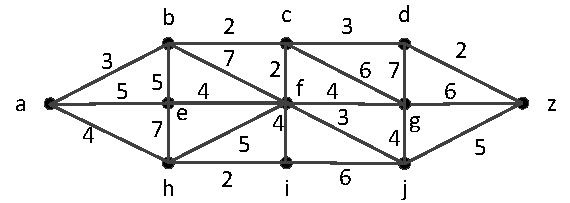
\includegraphics[width=96.3mm]{tut11p17_1}
            \end{figure}
            \emph{Find the length of a shortest path and a shortest path between each pair of
vertices in the weighted graph. 1) a,f.}\\$\;$\\\pause
            The answer is 7;(a, b, c, f). \qed
        \end{frame}


    \subsection{Problem 21}
        \begin{frame}[c]{\subsecname}
            \emph{Show that a tree is a bipartite graph.}\\$\;$\\\pause
            Let $T$ be a tree. Root $T$ at some arbitrary vertex. Let $V$ be the set of vertices on even levels and let $W$ be the set of vertices on odd levels. Since each edge is incident on a vertex in $V$ and a vertex in $W$, $T$ is a bipartite graph.\qed
        \end{frame}



    \subsection{Problem 23}
        \begin{frame}[c]{\subsecname}
            \emph{Show that a graph $G$ with $n$ vertices and fewer than $n-1$ edges is not connected.}\\$\;$\\\pause
%            Suppose that $G$ is connected. Add parallel edges until the resulting graph $G^*$ has $n-1$ edges. Since $G^*$ is connected and has $n-1$ edges, by Theorem 9.2.3, $G^*$ is acyclic. But adding an edge in parallel introduces a cycle. Contradiction. \qed
            Prove by contradiction.\\
            If the graph is connected, we can find a spanning tree. \\That consists n vertices and n-1 edges. \\Contradiction.\qed
        \end{frame}



\section{Problems cont.}
    \subsection{Problem 26.1}
        \begin{frame}[c]{\subsecname}
            \emph{Find a spanning tree for each graph using depth-first and breadth-first search.}\\
            \begin{figure}
                \centering
                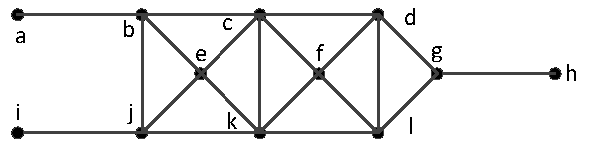
\includegraphics[width=99.6mm]{tut11p23_1_1}
            \end{figure}
%            \pause
%            \begin{figure}
%                \centering
%                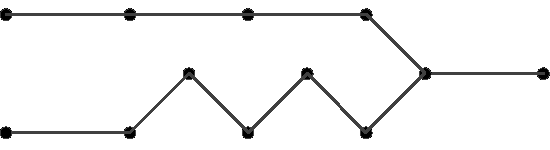
\includegraphics[width=93mm]{tut11p23_1_2} \qed
%            \end{figure}
        \end{frame}



    \subsection{Problem 27}
        \begin{frame}[c]{\subsecname}
            \emph{Let $T$ and $T^\prime$ be two spanning trees of a connected graph $G$. Suppose that an edge $x$ is in $T$ but not in $T^\prime$. Show that there is an edge $y$ in $T^\prime$ but not in $T$ such that $( T - \{ x \} ) \cup \{ y \} $ and $(T^\prime - \{ y \} ) \cup \{ x \} $ are spanning trees of $G$.}\\$\;$\\\pause
            Suppose that $x$ is incident on vertices $a$ and $b$. Removing $x$ form $T$ produces a disconnected graph with two components, $U$ and $V$. Vertices $a$ and $b$ belong to different components\--- say, $a \in U$ and $b \in V$. There is a path $P$ from $a$ to $b$ in $T^\prime$. As we move along $P$, at some point we encounter an edge $y=(v,w)$ with $v \in U$, $w \in V$. Since adding $y$ to $T-\{x\}$ produces a connected graph, $(T-\{x\}) \cup \{y\}$ is a spanning tree. Clearly, $(T^\prime-\{y\}) \cup \{x\}$ is a spanning tree. \qed
        \end{frame}
    

        
        

    \subsection{Homework Reminder}
        \begin{frame}<handout:0>[c]{\subsecname}
            \begin{itemize}[<+-|alert@+>]
            	\item Hardcopy is preferred. If you want to upload scanned softcopy to webct, make sure write Student ID on scanned paper. The multi-page pdf is best choice of the scaning format.
            	\item Answers are expected to be in increasing order. If not, please mark very clearly.
            	\item Check the problems carefully, especially the questions. Sometimes you have to prove your answer or draw the graph.
            \end{itemize}
        \end{frame}
    
    \begin{frame}<handout:0>[c]{\secname}
        \centerline{\Large{Any questions?}}
    \end{frame}
    
    
    
\end{document}



